% !TeX spellcheck = fr_FR
\documentclass[../main.tex]{subfiles}

\begin{document}

\subsection{Données synthétiques}\label{ssec:synthResults}

Les modèles ont été entraînés sur des jeux de données synthétiques générées à partir d'un processus de Hawkes linéaire à noyau exponentiel, en utilisant la librairie \verb|tick| pour Python \cite{2017arXiv170703003B}.

Un premier indicateur pour voir si le modèle peut retrouver la structure d'un Hawkes est de regarder la distribution du nombre d'événements, au total $N_T$ et par type d'événement $N^k_T, k\in\llbracket 1,K\rrbracket$. Réaliser le graphe de l'intensité $\lambda_t$ pour une séquence d'événements simulée permet aussi de voir si les phénomènes d'auto-excitation sont reflétés.

On a utilisé deux jeux de données synthétiques.

Le premier jeu de données est un processus de Hawkes en dimension $K=1$ avec $\mu=1$, $\alpha = \num{0.2}$, $\beta = \num{3.0}$ et $T = \num{80}$ (en secondes). Le nombre d'événements attendu est $T/(1-\alpha) = \num{100}$.

\paragraph{Decay-RNN}
Le modèle Decay-RNN réussit à répliquer correctement le comportement d'un processus de Hawkes en dimension 1, comme l'illustrent la distribution de $N_T$ \cref{fig:hawkes1DDecayRNNlengthDistrib} et le graphe de l'intensité \cref{fig:hawkes1DRNNintensityPlot}, qui sont réalisés pour $D=6$.\footnotemark

\footnotetext{Les séquences d'événements sont ici générées <<~à froid~>>, c'est-à-dire que l'on ne démarre pas le tirage des trajectoires avec une intensité de base. La seule information donnée au départ est un état caché $h(0)\sim \mathcal{N}(0, 0.01)$.}

\begin{figure}[htp]
	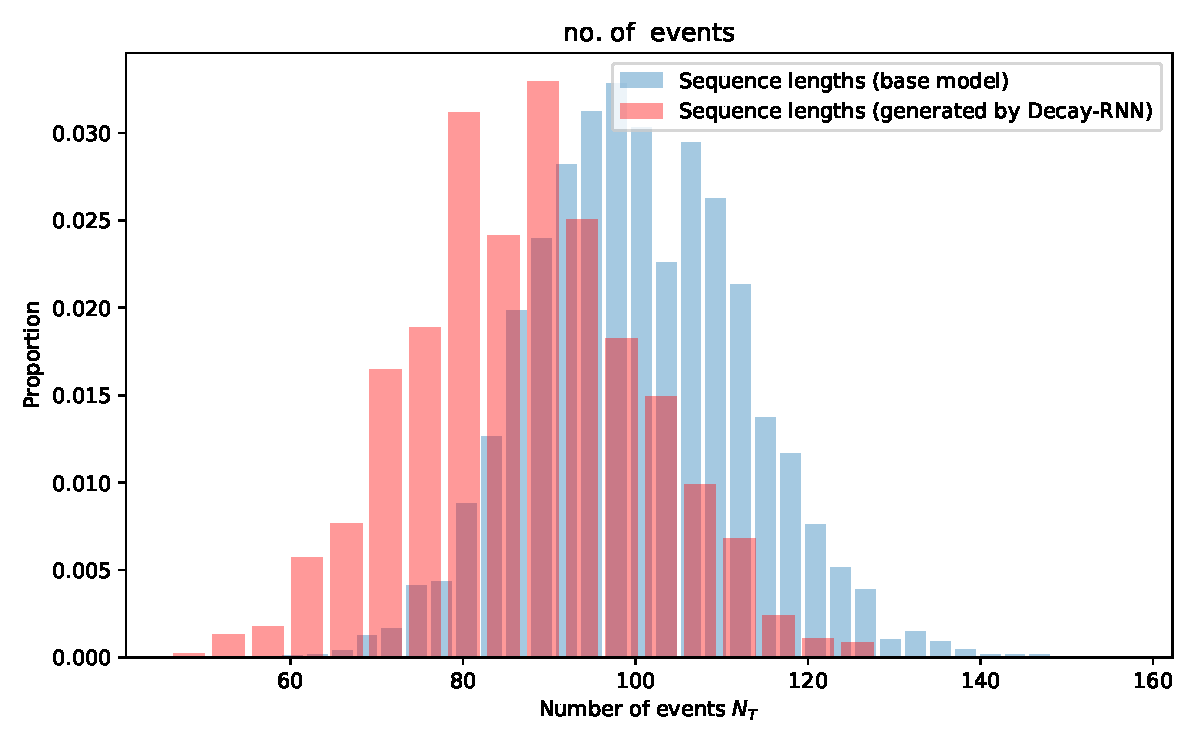
\includegraphics[width=\linewidth]{../results/seq_length_distrib_Decay-RNN-1d-hidden_8-20181202-140621.pdf}
	\caption{Distribution du nombre d'événements. $K=1$ type d'événements. Hawkes vs. Decay-RNN avec $D=6$ neurones cachés.}\label{fig:hawkes1DDecayRNNlengthDistrib}
\end{figure}

\begin{figure}[htp]
	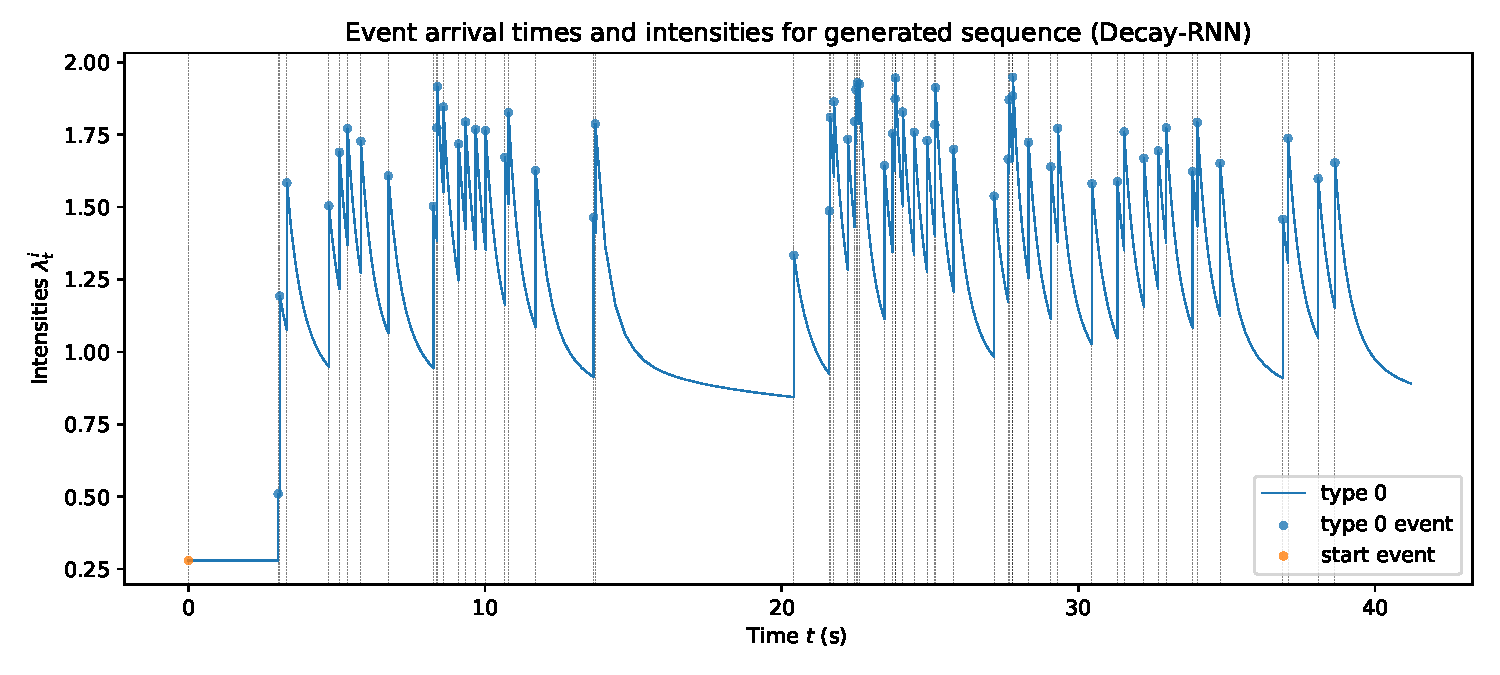
\includegraphics[width=\linewidth]{../results/intensity_Decay-RNN_1d_hidden8_20181202-140621.pdf}
	\caption{Processus d'intensité et temps d'arrivée. Trajectoire générée par le réseau Decay-RNN avec $K=1$, $D=6$.}\label{fig:hawkes1DRNNintensityPlot}
\end{figure}

Cependant, cette propriété semble perdue lorsque l'on augmente la dimension du processus. Les \cref{fig:hawkes2DDecayRNNlengthDistrib,fig:hawkes2DDecayRNNintensityPlot} montrent que le calibrage du réseau sur des données tirées d'un Hawkes bidimensionnel donne un mauvais résultat: les séquences générées sont très souvent d'un seul type d'événement. Parfois, comme dans le cas \cref{fig:hawkes2DDecayRNNintensityPlotRareBehaviour}, le type d'événement généré peut changer.

Le nombre d'états cachés a une influence sur ces résultats. L'augmenter ne mène pas forcément à un meilleur résultat sur des données synthétiques (voir \cref{fig:hawkes1DDecayRNNlengthDistribHidden32} pour la distribution du nombre d'événements avec $D=24$).

\begin{figure}[htp]
	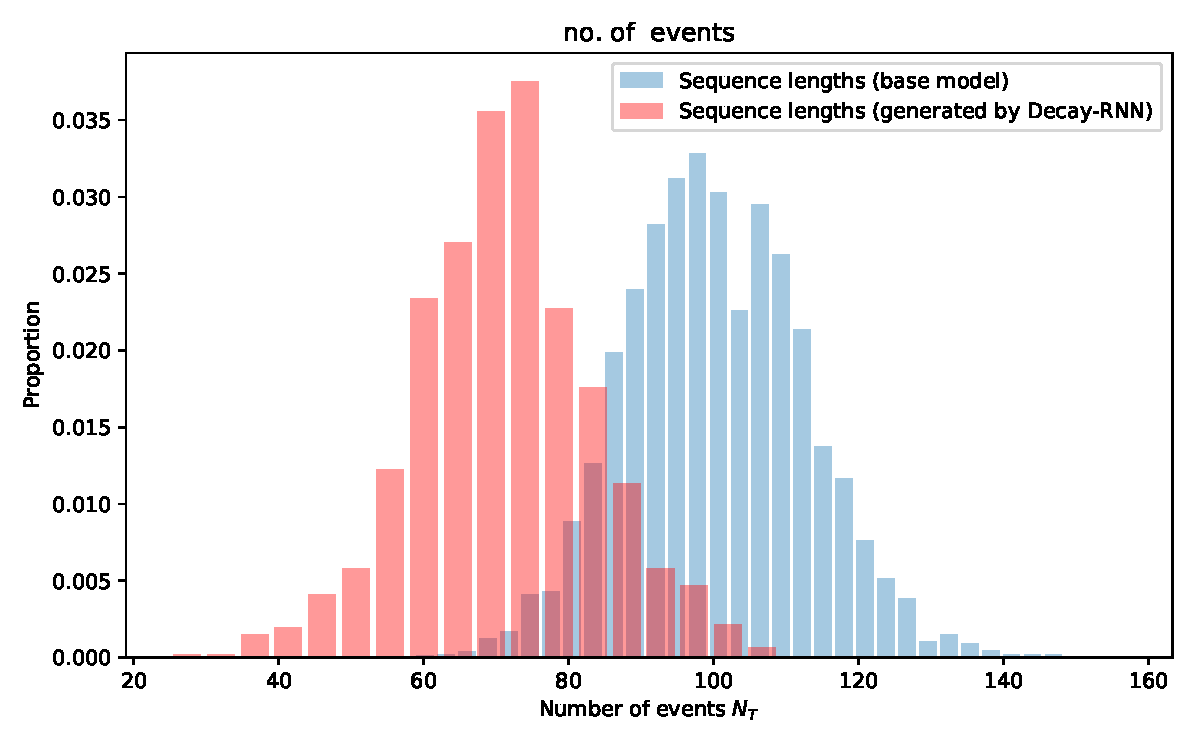
\includegraphics[width=\linewidth]{../results/seq_length_distrib_Decay-RNN-1d-hidden_32-20181202-141923.pdf}
	\caption{Distribution du nombre d'événements. Hawkes 1D vs. Decay-RNN avec $D=32$.}\label{fig:hawkes1DDecayRNNlengthDistribHidden32}
\end{figure}


\begin{figure}[htp]
	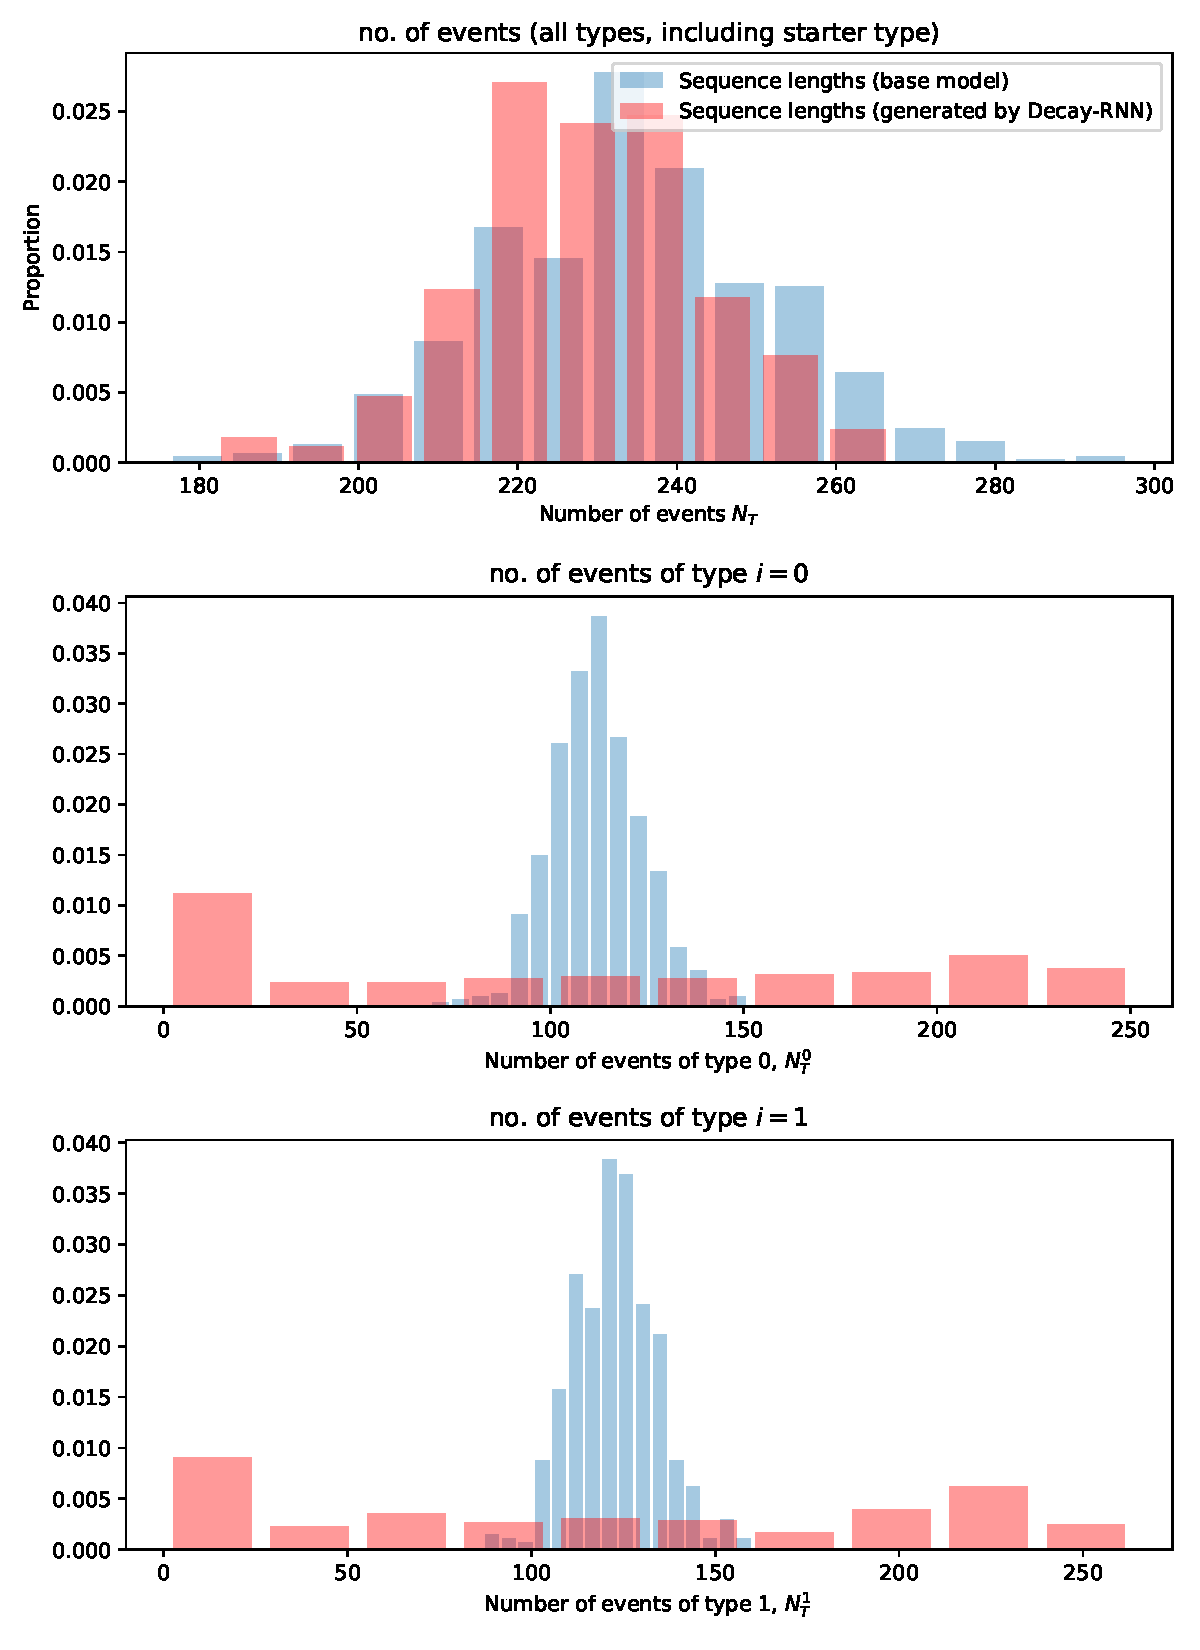
\includegraphics[width=\linewidth]{../results/seq_length_distrib_Decay-RNN-2d-hidden_12-20181201-003410.pdf}
	\caption{Distribution du nombre d'événements. Hawkes bidimensionnel vs. Decay-RNN avec $D=12$ neurones cachés. La distribution par type d'événement suggère que les séquences générées sont majoritairement d'un seul type à la fois.}\label{fig:hawkes2DDecayRNNlengthDistrib}
\end{figure}

\begin{figure}[htp]
	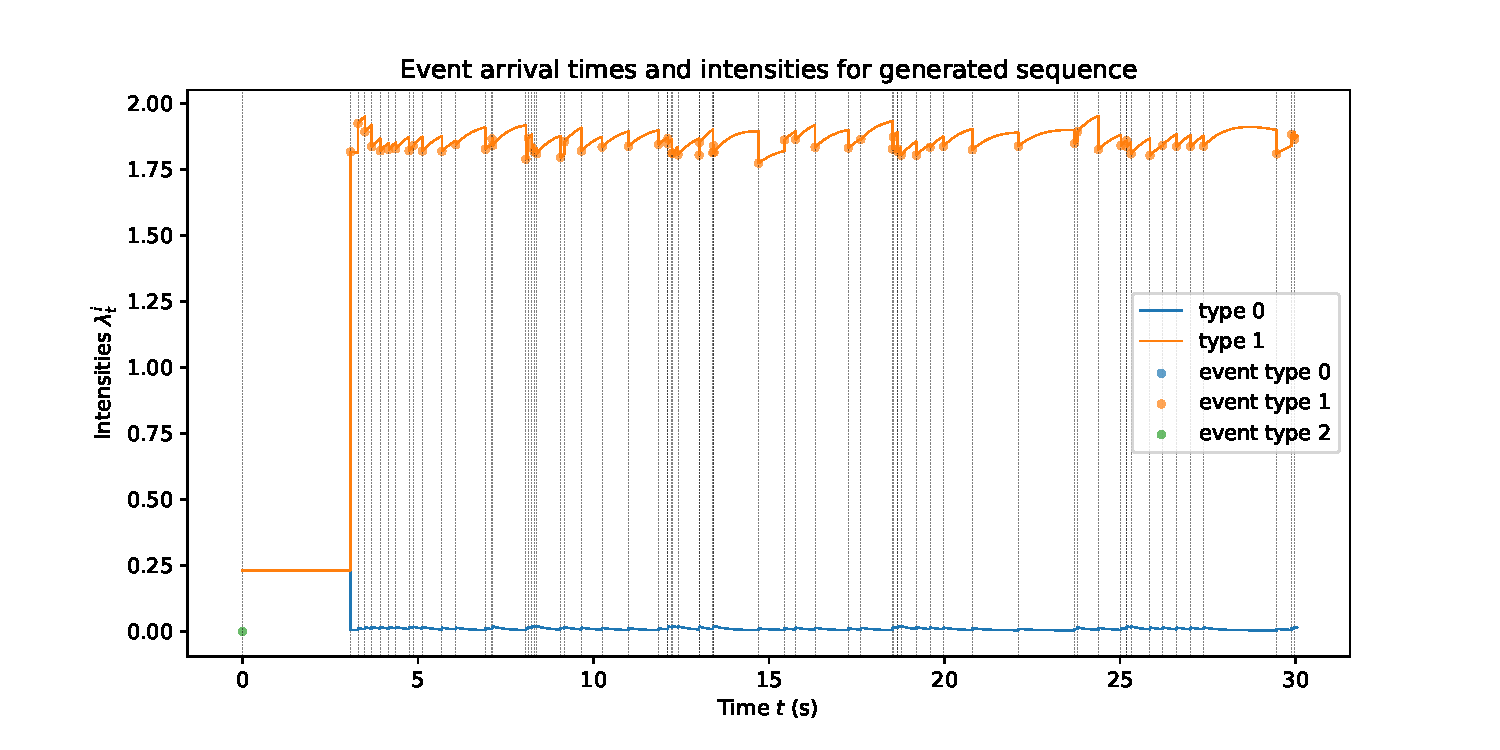
\includegraphics[width=\linewidth]{../results/intensity_Decay-RNN_2d_hidden12_20181201-003410.pdf}
	\caption{Trajectoire d'intensité générée par Decay-RNN en dimension 2 avec $D=12$. On observe un saut immédiat de l'intensité des événements de type 1 et l'annulation de celle de l'autre type.}\label{fig:hawkes2DDecayRNNintensityPlot}
\end{figure}

\begin{figure}[htp]
	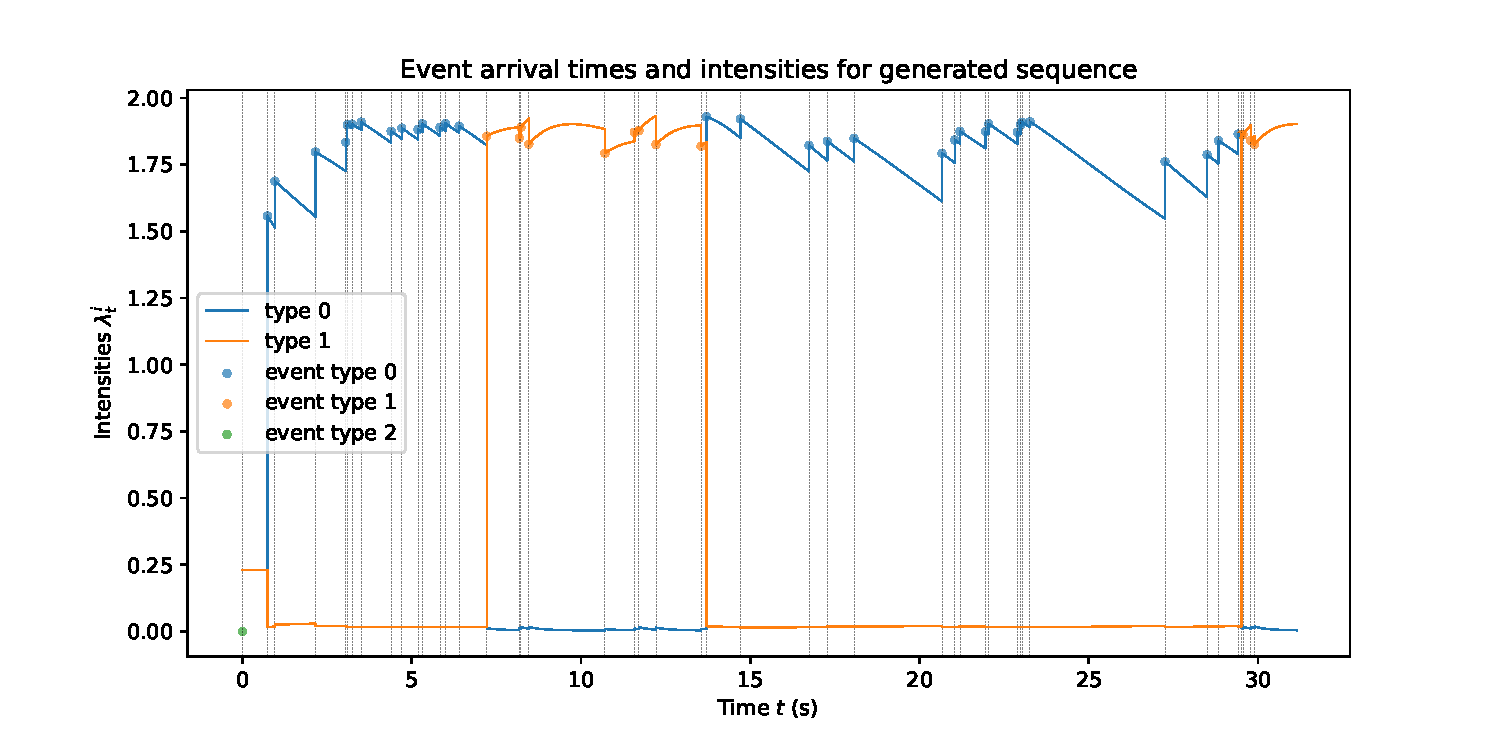
\includegraphics[width=\linewidth]{../results/intensity_Decay-RNN_2d_hidden12_20181201-003410_RARE_TYPESWITCH.pdf}
	\caption{Trajectoire d'intensité générée par Decay-RNN en dimension 2 avec $D=12$. Pour le réseau Decay-RNN, le comportement où le type des événements générés change est en fait assez rare. Le comportement <<~tout ou rien~>> de \cref{fig:hawkes2DDecayRNNintensityPlot} est beaucoup plus courant.}\label{fig:hawkes2DDecayRNNintensityPlotRareBehaviour}
\end{figure}



\end{document}